\section{Pré-processamento} 

\begin{frame}
    \frametitle{Pré-processamento de Dados}
    \begin{itemize} 
        \item Dados reais podem conter valores ausentes, variáveis desbalanceadas ou ruídos.
        \item Preparação, organização e estruturação dos dados.
        \item Modelos de ML requerem dados bem formatados.
    \end{itemize}

    \begin{center}
    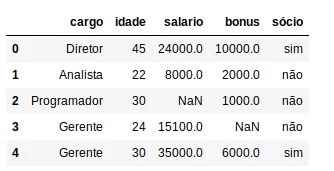
\includegraphics[width=0.6\linewidth]{img/tabelaintropre.jpg}
    \end{center}

\end{frame}

\begin{frame}
    \frametitle{Técnicas}
    \begin{itemize} 
        \item Codificação de variáveis categóricas 
        \item Padronização
        \item Normalização
        \item Divisão dos dados
    \end{itemize}
\end{frame}

\begin{frame}
    \frametitle{Codificação de variáveis categóricas}
    Utilizadas para converter variáveis categóricas em uma forma numérica que possa ser utilizada por modelos de Machine Learning.

    \vspace{0.3cm}
    
    \begin{itemize}
        \item Label Encoder.
        \item One Hot Encoder.
    \end{itemize}
\end{frame}

\begin{frame}{Label Encoder}
    \begin{itemize}
        \item Converte variáveis categóricas em valores inteiros.
        \item Ideal para categorias com uma ordem (variáveis ordinais).
    \end{itemize}

    \begin{center}
    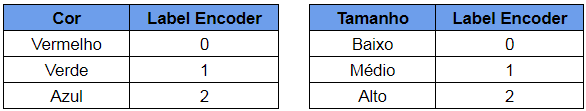
\includegraphics[width=0.8\linewidth]{img/LabelEncoder2.png}
    \end{center}

    \begin{center}
    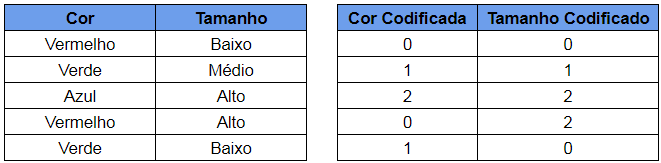
\includegraphics[width=0.8\linewidth]{img/LabelEncoder.png}
    \end{center}
\end{frame}

\begin{frame}{One Hot Encoder}
    
    \begin{itemize}
        \item Cria uma nova variável binária (0 ou 1) para cada categoria única da variável original.
        \item Ideal para um número reduzido de categorias e variáveis nominais.
    \end{itemize}
    
    \begin{center}
    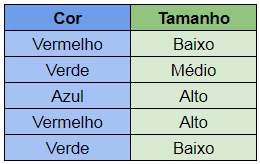
\includegraphics[width=0.3\linewidth]{img/One Hot 2.png}
    \end{center}

    \begin{center}
    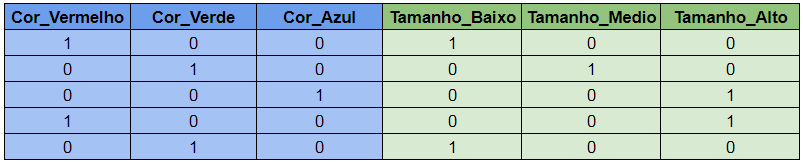
\includegraphics[width=0.8\linewidth]{img/One Hot.png}
    \end{center}
\end{frame}


\begin{frame}
    \frametitle{Padronização (Z-Score)}
    \begin{itemize}
    \setlength{\itemsep}{6pt}
        \item  Os dados são transformados de acordo com a distribuição estatística.
        \item Utiliza a Média e o Desvio Padrão.
        \item Menos sensível a outliers (valores extremos).
        \item Pode resultar em valores negativos.
    \end{itemize}
    
    \begin{center}
        \[
        X' = \frac{x - \mu}{\sigma}
        \]
    \end{center}
    
\end{frame}

\begin{frame}{Padronização}
    Padronização para o exemplo anterior
    \begin{itemize}
        \item Média (\(\mu\)): 41.0
        \item Desvio padrão (\(\sigma\)): 19.97
    \end{itemize}
    \vspace{0.3cm}
    \centering
  \begin{center}
    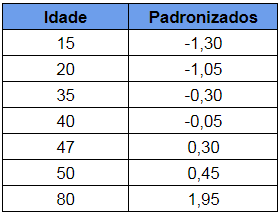
\includegraphics[width=0.4\linewidth]{img/Padronização.png}
    \end{center}
\end{frame}

\begin{frame}
    \frametitle{Normalização}
    
    \begin{itemize}
    \setlength{\itemsep}{10pt}
         \item Usado para reescalar os valores dos dados para que fiquem dentro de um intervalo específico, geralmente entre 0 e 1.
         \item Garante que todas as variáveis tenham a mesma escala.
         \item Evita que variáveis com valores maiores influenciem de forma desproporcional o modelo de Machine Learning.
     \end{itemize}
\end{frame}

\begin{frame}
    \frametitle{Normalização Min-Max}
    \begin{itemize}
    \setlength{\itemsep}{10pt}
         \item Um exemplo de normalização min-max é a conversão de idades de um grupo de pessoas para um intervalo entre 0 e 1.
        \item Se as idades são 15, 20, 35, 40 e 50 anos, o valor mínimo é 15 e o máximo é 50.
     \end{itemize}

    \begin{figure}[h!]
    \centering
    \begin{minipage}{0.45\textwidth}
        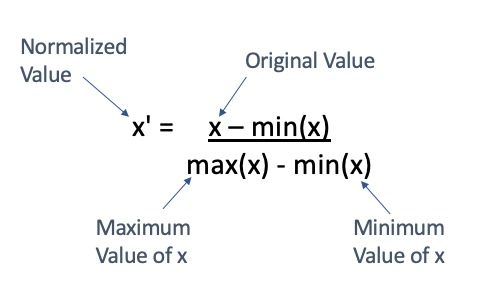
\includegraphics[width=1\linewidth]{img/minmax.jpg}
    \end{minipage}
    \begin{minipage}{0.45\textwidth}
        \centering
          \begin{center}
    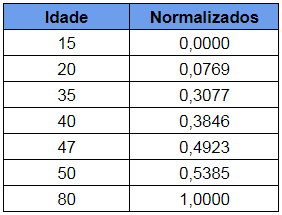
\includegraphics[width=0.8\linewidth]{img/Normalização.png}
    \end{center}
    \end{minipage}
    \end{figure}
     
\end{frame}

\begin{frame}
    \frametitle{Divisão dos dados}
    \begin{itemize}
    \setlength{\itemsep}{6pt}
        \item \textbf{Treinamento:} Usado para ajustar os parâmetros do modelo.
        \item \textbf{Validação:} Usado para avaliar o desempenho do modelo e dos hiperparâmetros durante o treinamento.
        \item \textbf{Teste:} Usado para avaliar a performance final do modelo em dados não vistos durante o treinamento.
    \end{itemize}

    \begin{figure}
        \centering
        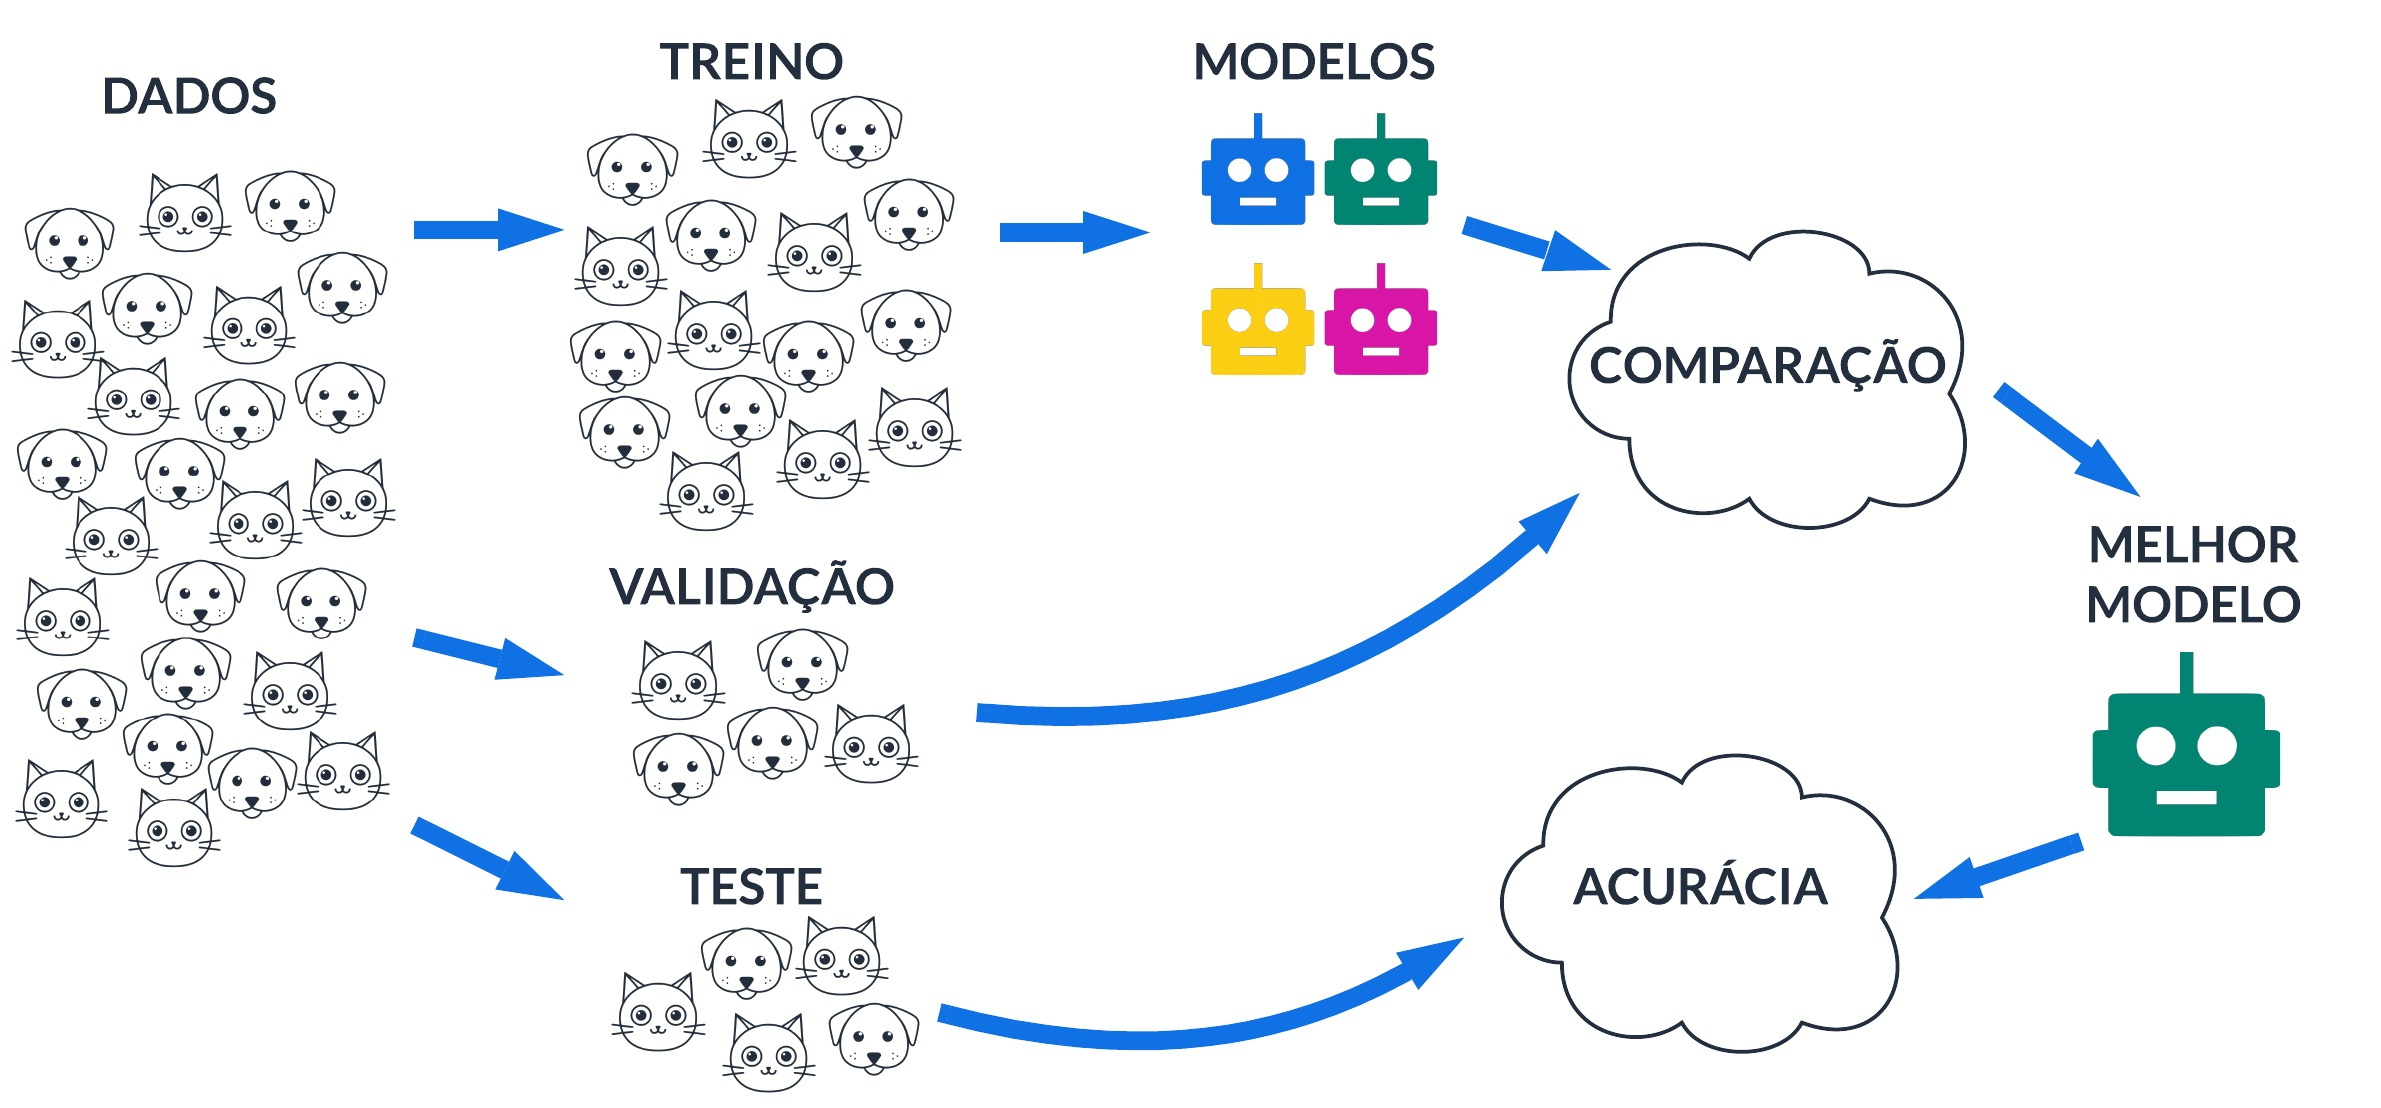
\includegraphics[width=0.7\linewidth]{img/image-ttv.png}
    \end{figure}
\end{frame}

\begin{frame}
    \frametitle{Divisão dos dados}

    Divisão mais comum dos dados que pode variar com base no desempenho do modelo:
    
    \vspace{0.3cm}
    
    \begin{itemize}
    \setlength{\itemsep}{6pt}
        \item \textbf{Treinamento:} 70\% - 80\% dos dados.
        \item \textbf{Validação:} 10\% - 15\% dos dados.
        \item \textbf{Teste:} 10\% - 15\% dos dados.
    \end{itemize}
\end{frame}